%!TEX root = /Users/gilesb/UofC/thesis/phd-thesis/phd-thesis.tex
\chapter{Transformations of Quantum Programs}\label{chap:transformations_of_quantum_programs}



\section{Subroutines} % (fold)
\label{sec:subroutines}
In the following, we will assume \emph{gate} as above is a given
and that $W\subset\nat$ is fixed and  finite. We
will use typing notation to show membership in $W$ --- $w\in W$
is equivalent to $w::W$.


\subsection{Definition of a Subroutine} % (fold)
\label{sub:definition_of_a_subroutine}
The concept of \emph{subroutine} as defined below is intended
to capture the essence of a describable computation
in a quantum language. The low level subroutine is considered in
isolation, meaning that it contains no information regarding
how it fits into a larger circuit.

\begin{definition}\label{def:bare_subroutine}
  A \emph{bare subroutine} is defined as a list of gates, written as
   $[g_0,g_1,\ldots,g_{n}]$. The list of
  gates must satisfy the following:
  \begin{itemize}
    \item $\rng{g_i} = \dom{g_{i+1}}$ for $i\in\{0,1,\ldots,n-1\}$.
  \end{itemize}
\end{definition}

A bare subroutine $B$ can then be viewed as a function from $\dom{g_0}$
to $\rng{g_n}$ by
applying each gate in order to $\dom{g_0}$.

\begin{definition}\label{def:low_level_subroutine}
  A \emph{low level subroutine} is a bare subroutine with a
  triple $(C,I,O)$ where each of $C,I,O$ are of type \type{Arity} and
  \begin{align}
    \dom C \cap \dom I &= \phi\\
    \dom C \cap \dom O &= \phi
  \end{align}
\end{definition}

In the definition of the low level subroutine, the triple $(C,I,O)$
describes the inputs and outputs of the subroutine. $C$
describes the control wires, which are inputs and outputs without
change, $I$ the input wires and $O$ the output wires.


The above data together with three additional flags provides
everything we need to know regarding a subroutine:
\begin{definition}\label{def:subroutine}
  A \emph{subroutine} is a low level subroutine together with a tripartite
  flag $c$ with values in $\{N,B,Q\}$, and two boolean flags, $r$ and $n$.
\end{definition}
The three flags describe the ways this subroutine may be used. Each of
these flags
provide information that the calling quantum program uses to
determine the ways the subroutine may be called:
\begin{itemize}
  \item \emph{Controllable}: When $c$ is $B$, a calling program may make this
  subroutine the target of one or more \emph{control wire}s with type \bit.
  When $c$ is $Q$, the control wires my be of type \bit or \qubit.
  When $c$ is $N$, no control wires may be used. Note this is separate from
  the $C$ wires of the subroutine, which may be used for internally
  controlling portions of the subroutine.
  \item \emph{Reversible}: A calling program may specify the
  subroutine run normally or reversed.
  \item \emph{No-controllable}: In the case where this subroutine is
  part of a preparation / unpreparation in a (prep, transform, unprep)
  sequence and that sequence is controlled, then the control wires may
  be ignored for this subroutine.
\end{itemize}

Noting that the domains of $C$ and $I$ and the domains of $C$ and $O$ do
not overlap, we can also provide an ordering of the inputs and outputs for
a low level subroutine. This ordering is used for display purposes and
has no additional semantic content.

\begin{definition}\label{def:low_level_subroutine_ordering}
  An \emph{ordering} of a low level subroutine is a pair of bijections,
  $(i,o)$ such that:
  \begin{align}
    i: \dom C \cup \dom I \leftrightarrow \{0,1,\ldots,n-1\}\\
    o: \dom C \cup \dom O \leftrightarrow \{0,1,\ldots,m-1\}
  \end{align}
  where $|\dom C \cup \dom I| = n$ and $|\dom C \cup \dom O| = m$.
\end{definition}

% subsection definition_of_a_subroutine (end)


\subsection{Subroutine Calls} % (fold)
\label{sub:subroutine_calls}

In this section, we describe the permissible bindings given two
sets of wires, where the first set will be considered as control wires and
the second as either input or output wires.
\begin{definition}\label{def:permissible_bindings}
  Given $C$ and $K$ are \type{Arity}
  functions over the same set of typed wires $V$,
  then $f$ is a \emph{permissible binding} to a
  set of typed wires $W$ with \type{Arity} $T_w$ when:
  \bi
  \item $f: \dom C + \dom K \to W$,
  \item $\forall x, y\in \dom f, f(x)=f(y) \implies x=y \vee x,y\in \dom C$,
  \item $x\in \dom C \wedge C(x) = \qubit
  \implies T_w(f(x)) = \bit \vee T_w(f(x)) = \qubit$,
  \item $x\in \dom C \wedge C(x) = \bit \implies T_w(f(x)) = \bit$,
  \item $x\in \dom K  \implies T_w(f(x)) = K(x)$.
  \ei
\end{definition}

We denote the permissible bindings to $W$ of $C$ and $K$ by $F(C,K,W)$.

\begin{definition}\label{def:subroutine_call}
  In a context of typed wires $W_1$,
  a \emph{subroutine call}, resulting in the typed wires $W_2$,
  of the subroutine $([gates],C,I,O,r,c,n)$
  is a tuple $(f,g,h,i,ncf,ctrls)$ consisting of three functions,
  two boolean flags and a list of control wires.
  The functions $f,g,h$ must satisfy:
  \bi
  \item $f:\dom C \to W_1 \cap W_2$
  \item $g:\dom I \to W_1$
  \item $h:\dom O \to W_2$
  \item $f + g \in F(C,I,W_1)$
  \item $f + h \in F(C,O,W_2)$.
  \ei
  The two flags must satisfy:
  \bi
  \item $i \implies r$
  \item $ncf \implies n$.
  \ei
  The control list must satisfy:
  \begin{itemize}
    \item $\forall w_c \in ctrls, \text{fst}(w_c) \in W_1 \cap W_2$,
    \item $N = c \implies \text{length}(ctrls) = 0$,
    \item $B = c \implies \forall w_c \in ctrls, T_1(\text{fst}(w_c)) = \bit$.
  \end{itemize}
\end{definition}


% subsection subroutine_calls (end)

\subsection{High Level Structure} % (fold)
\label{sub:high_level_structure}

Let $s,t$ be of type of the family \type{QCData}
and $a$ be of shape $s$, $b$ be of shape $t$.
Further, let $A = \{qt|qt::a, qt \text{ has shape }s\}$
and $B = \{qt|qt::b, qt \text{ has shape }t\}$, that is,
$A$ and $B$ are the sets of quantum terms of shape $s$
(respectively $t$) and type $a$ (respectively $b$).

\begin{definition}\label{def:high_level_structure}
  A \emph{high level structure} for a call to the subroutine
  $([gates],C,I,O,r,c,n)$ starting in context $W_1$ and
  ending in context $W_2$ is a
  pair of maps $(i_s,o_s)$ with $i_s:A \to F(C,I,W_1)$
  and $o_s:F(C,O,W_2)\to B$.
\end{definition}

\begin{definition}\label{def:structured_subroutine_call}
  Given the data for a subroutine call as above in 
  \vref{def:subroutine_call}, a \emph{structured subroutine call} is a
  high level structure as in \vref{def:high_level_structure}
  and a pair of quantum terms $(a,b)$ such that:
  \begin{itemize}
    \item $i_s(a) = f+g$ and
    \item $o_s(f+h) = b$.
  \end{itemize}

\end{definition}

% subsection high_level_structure (end)

% section subroutines (end)

\section{Subroutine Calls and Transformers} % (fold)
\label{sec:subroutine_calls_and_transformers}

We are interested in two transformed calls of subroutines. Iteration and
folding. We provide the necessary information for creating either a
transformed call or first transforming the subroutine and then doing a
standard call as in \vref{sub:subroutine_calls}.

\subsection{Iteration} % (fold)
\label{sub:iteration}
Iteration of subroutines means to call the same subroutine
within a quantum circuit some positive number of times.
Discussion points:
\begin{itemize}
  \item Can we handle the case of zero iterations? Would this
  just mean doing a direct mapping of the I to the O
  in numerical sequence?
  \item Can we handle the case of negative iterations? This could
  mean calling the inverse of the subroutine in the case
  where it is reversible and then iterating.
  \item Does iteration affect the no-control or other flags?
  \item The analysis below assumes that ``non-linear safety'' is
  an important property to preserve during iteration.
  If we remove that requirement, iteration becomes more flexible,
  e.g., the bijections $c_b$ and $io_b$ could be
  replaced with a single bijection $cio_b : C\cup O \leftrightarrow C\cup I$.
  This would allow a \qubit that was
  affected by the subroutine on one iteration to be used as the
  control on the next iteration. (Or is this the simple
  case that has already been handled?)
\end{itemize}
\begin{definition}\label{def:iterated_subroutine_call}
  Given a subroutine as in \vref{sub:subroutine_calls},
  and a subroutine call $(f,g,h,i,ncf,ctrls)$
  an \emph{iterated call} of the subroutine
  $S = ([gates],C,I,O,r,c,n)$ consists of all elements of a
  subroutine call excepting $f$ plus another
  tuple of five elements $(f_{in},f_{out},c_b,io_b,i_{count})$
  where:
  \begin{itemize}
    \item $f_{in}:\dom C \to W_1\cap W_2$
    \item $f_{out}:\dom C \to W_1\cap W_2$
    \item $i_{count}$ is a positive integer,
    \item $c_b$ is a bijection (permutation) of $C$ to $C$,
    \item $io_b$ is a bijection between $I$ and $O$.
    \item $f_{in}+ g \in F(C,I,W_1)$
    \item $f_{out}+ h \in F(C,O,W_2)$
    \item The relation $f_{out} \circ c_b^{i_{count}} \circ f_{in}^{-1}$
    is a function.
  \end{itemize}
  Note these requirements mean that $|I| = |O|$.
\end{definition}

\begin{definition}\label{def:structured_iterated_call}
  Given the data for an iterated call,
  a \emph{structured iterated call} is a high level structure as in
  \vref{def:high_level_structure} and a pair of quantum
  terms $(a,b)$ such that:
  \begin{itemize}
    \item $i_s(a) = f_{in}+g$ and
    \item $o_s(f_{out}+h) = b$.
  \end{itemize}

\end{definition}

From the definition, note the $C$ wires may be permuted as
desired, but the combination of the $f_{in}^{-1}$ and
the permutation must leave the wires in a state where $f_{out}$
is well-defined. See below for an example.
Note the disposition of the wires due to calling the iterated
subroutine is given by:
\begin{itemize}
  \item Control mapping: $f_{out} \circ c_b^{i_{count}}\circ f_{in}^{-1}$,
  \item In-out mapping: $h \circ io_b^{i_{count}} \circ g^{-1}$.
\end{itemize}


\begin{example}[Single call]
\end{example}
  For this example, we will elide the details relating to high level
  structure, invertability, control wires and the no-control flag.

  Suppose $C=[c_1,c_2,c_3], I=[i_1,i_2]$ and $O=[o_1,o_2]$.
  For the first part of the example, assume we are calling $S$
  from a context of $W_1=[w_1,w_2,w_3,w_4]$, resulting in the
  same context (i.e., $W_1 = W_2$).
  In this case, the call of $S$ can be given by:
  \begin{itemize}
    \item $f = \{c_1\mapsto w_1, c_2 \mapsto w_1, c_3 \mapsto w_4\}$,
    \item $g = \{i_1 \mapsto w_2, i_2 \mapsto w_3\}$
    \item $h = \{o_1 \mapsto w_3, o_2 \mapsto w_2\}$
  \end{itemize}
  Hence we are calling $S$ which will use $w_1$ as its
  first two control inputs and $w_4$ as the third. The
  inputs will use $w_2$ and $w_3$, while the output will
  ``switch'' those to $w_3$ and $w_2$.

\begin{example}[Iterated call]
\end{example}
Assume $S$ is as above and we are using the call as above.
To aid in distinguishing input and output wires of the calling circuit,
we will use $w'$ for naming the output wires, so we may write
$W_1 = [w_1,w_2,w_3,w_4]$ and $W_2=[w'_1,w'_2,w'_3,w'_4]$, noting that
$w_i = w'_i$ for $i\in\{1,2,3,4\}$. A call iterated 5 times of
$S$ is $(g,h,i,ncf,ctrls)$ plus
the tuple $(f_{in},f_{out},c_b,io_b,5)$ where
\begin{itemize}
  \item $f_{in} = \{c_1\mapsto w_1, c_2 \mapsto w_1, c_3 \mapsto w_4\}$,
  \item $f_{out} = \{c_1\mapsto w'_4, c_2 \mapsto w'_1, c_3 \mapsto w'_1\}$,
  \item $c_b = (c_1,c_2,c_3)$,
  \item $io_b = \{o_1\mapsto i_2, o_2\mapsto i_1\}$
\end{itemize}
If we calculate the movement of the wires for this iterated call, we see
\begin{align}
  (w_1,w_4)\xrightarrow{f_{in}^{-1}} &C=(w_1,w_1,w_4) \xrightarrow{(1,2,3)^5}
    C=(w_4,w_1,w_1) \xrightarrow{f_{out}} (w'_1(=w_1),w'_4(=w_4))\\
  (w_2,w_3)\xrightarrow{g^{-1}} &I=(w_2,w_3) \xrightarrow{io_b^5\circ S}
    O=(w_3,w_2) \xrightarrow{h} (w'_3(=w_3),w'_3(=w_3))
\end{align}


In this above example, the choice of $f_{in}$ and $f_{out}$
worked correctly with $c_b$ such that the mappings were
well defined. Consider however, if $f_{out}$ were defined
as $\{c_1\mapsto w'_1, c_2 \mapsto w'_1, c_3 \mapsto w'_4\}$.
We would then be expected to map / combine $w_1$ and $w_4$
into $w'_1$ and duplicate $w_1$ into both $w'_1$ and $w'_4$.


% subsection iteration (end)

\subsection{Iteration transformation of a subroutine} % (fold)
\label{sub:iteration_transformation_of_a_subroutine}

The data required to transform a subroutine is similar to that of an iterated
subroutine call.

\begin{definition}\label{def:iteration_transform}
  The \emph{iteration transform} of a subroutine is a function $S_i$ with
  parameters $(n,c_p,io_b)$ which takes the subroutine $(gates,C,I,O,r,c,n)$
  to the subroutine $(gates',C',I',O',r,c,n)$.
  The parameters have the following types:
  \begin{align*}
    n&::\type{Int}, n>0;\\
    c_p&::\type{Perm_C}, \text{Permutations of the elements of }C\\
    io_b&::\type{bijection(I\leftrightarrow O)}
  \end{align*}
\end{definition}

The function $S_i$ performs the following actions:
\begin{itemize}
  \item Type checking:
  \begin{itemize}
    \item Ensure  $c_p$ is a permutation of the appropriate number of wires.
    \item Ensure $n$ is a positive number greater than 0.
    \item Ensure $io_b$ is a bijection between the $O$ and $I$ wires.
  \end{itemize}
  \item Create $n$ copies of $gates$.
  \item Connect the $O$ wires or copy $i-1$ to the $I$ wires of copy $i$,
  using the bijection $io_b$.
  \item Apply the permutation $c_p$ to the $C$ out wires of copy $i-1$
  and connect to the input $C$ wires of copy $I$.
  \item Apply the permutation $c_p^k$ to the $C$ out wires of copy $n$
  where $c_p^{n-1+k} = Id$. Connect those wires to the $C'$ output.
  \item Connect the $C'$ input wires to the $C$ input wires of copy 1.
  \item Connect the $I'$ wires to the $I$ wires of copy 1.
  \item Connect the $O$ wires of copy $n$ to the $O'$ wires.
\end{itemize}

The intended effect of this transform may be seen in
\vref{fig:transforming_a_subroutine_to_an_iterated_subroutine}
\begin{figure}[htbp]
  \centering
     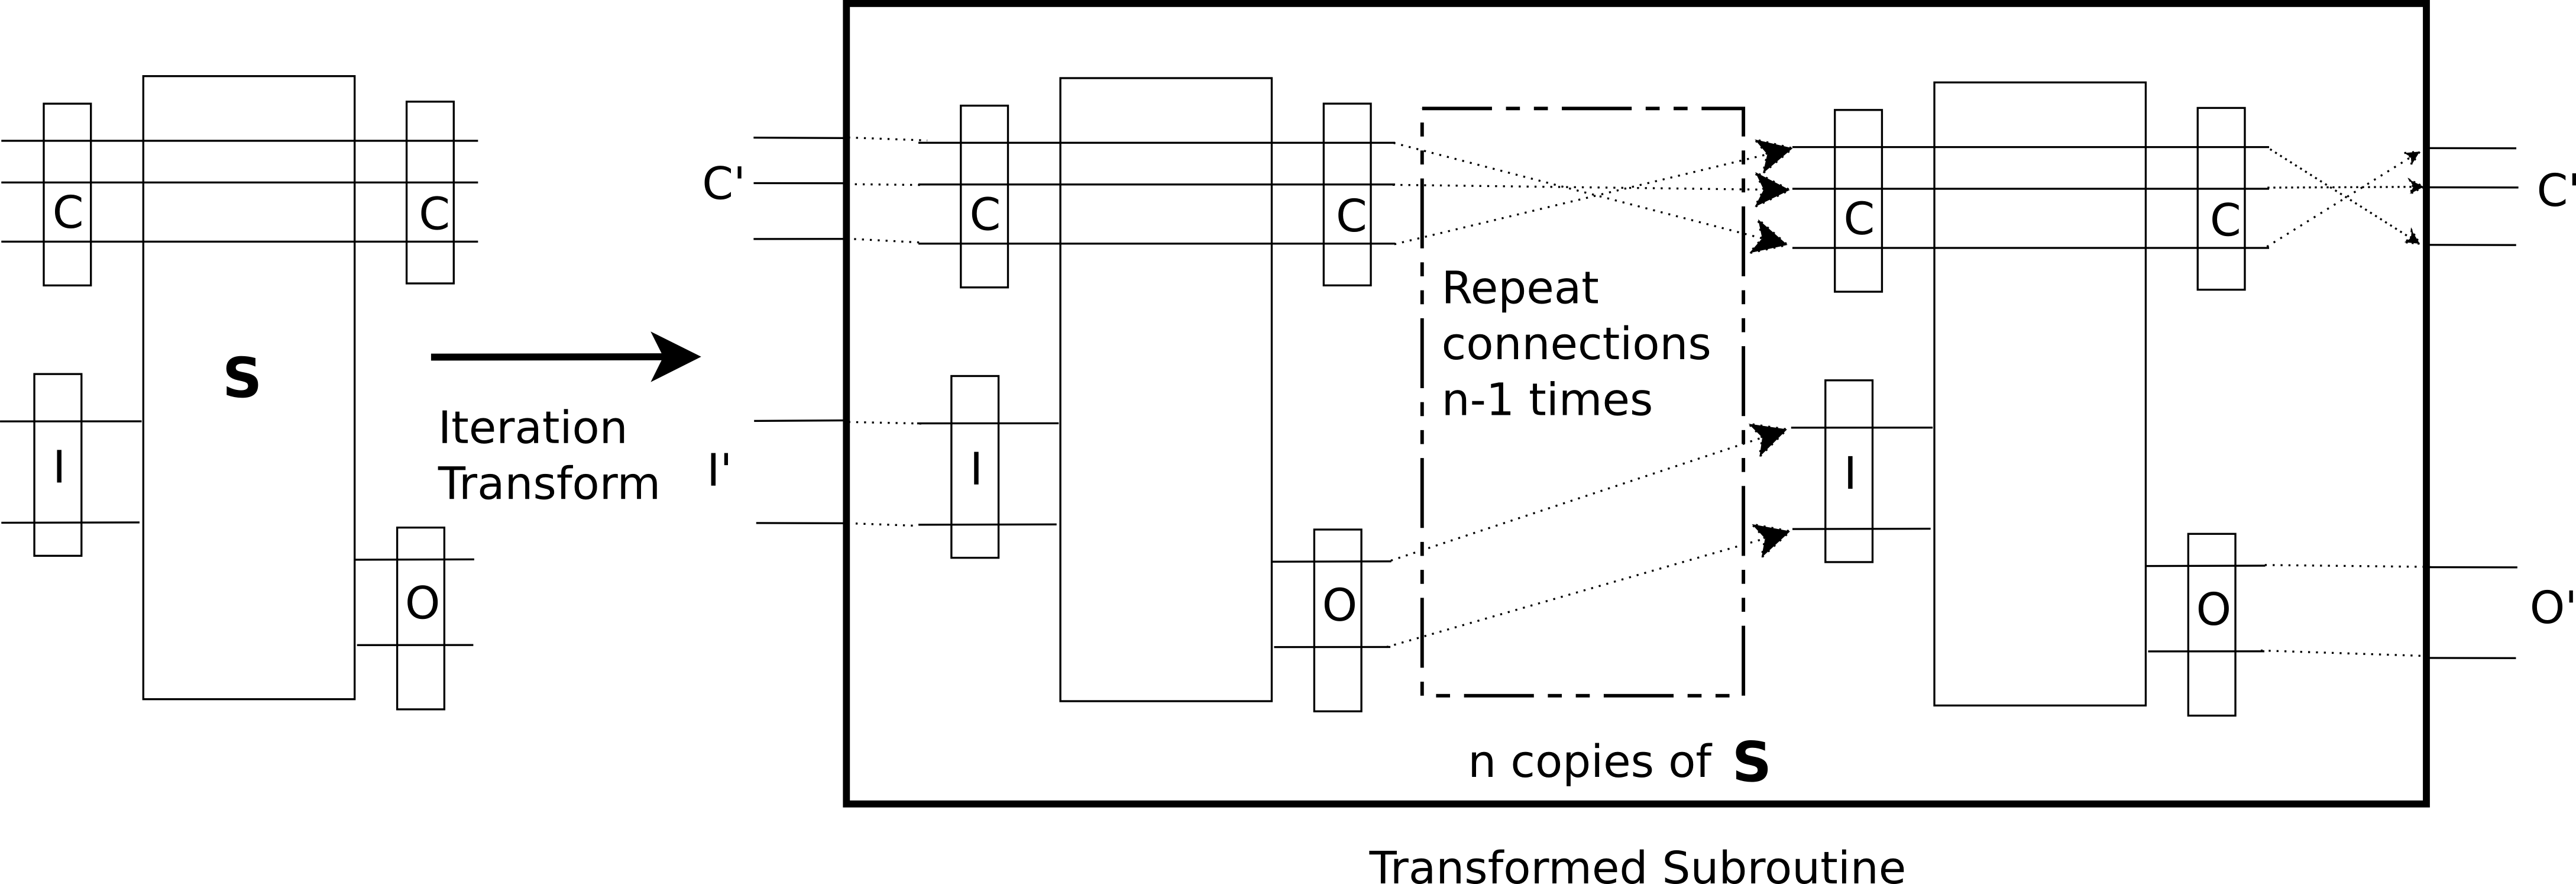
\includegraphics[scale=.4]{diagrams/SubroutineIterationTransform.png}
   \caption{Transforming a subroutine to an iterated subroutine}
   \label{fig:transforming_a_subroutine_to_an_iterated_subroutine}
\end{figure}
% subsection iteration_transformation_of_a_subroutine (end)

\subsection{Folding subroutines} % (fold)
\label{sub:folding_subroutines}

In addition to the concept of iteration the ability to fold
subroutines over data structures could also be useful. A
folded call of a subroutine is similar to an iteration, in
that controls and possibly some of the inputs
and outputs are iterated. The difference occurs in that we
expect to take some of the inputs from a data structure and
return some of the outputs to a data structure. An example of
this would be folding over a list of \qubit{s} where
each qubit is taken as a input for each iteration.

First, we will examine the requirements for a non-linear
safe fold, that is, where no input duplication on the
control wires is allow



\begin{definition}\label{def:linear_only_subroutine_fold}
  Given a subroutine $S=([gate],C,I,O,c,r,n)$, a starting context of
  typed wires $W_1$ and a data structure on wires $D\subset W_1$, a
  \emph{linear-only folded call} of $S$ over $D$ resulting in the context
  of typed wires $W_2$ and the data structure $E\subset W_2$ consists of the
  tuple $(CI_f,CO_f,  g, h, ciof_b, s_{in}, s_{out})$ where
  \begin{itemize}
    \item $CI_f::\type{Arity}, \dom{CI_f} \subset \dom{C}\cup \dom{I}$,
    \item $CO_f::\type{Arity}, \dom{CO_f} \subset \dom{C}\cup \dom{O}$,
    \item $g:\dom{C}\cup\dom I / \dom{CI_f} \to W_1$ and $g$ is injective,
    \item $h:\dom{C}\cup\dom O /\dom{CO_f} \to W_2$ and $h$ is injective
    \item $ciof_b$ is a bijection between $(\dom{C}\cup\dom{O})/\dom{CO_f}$
      and $(\dom{C}\cup\dom{I})/\dom{CI_f}$,
    \item $s_{in}: \dom{CI_f} \to W_1$ (pulls from $D$),
    \item $s_{out}: \dom{CO_f} \to W_2$ (pushes to $E$),
    \item $g + s_{in} \in F(\nothing,I,W_1)$,
    \item $ciof_b^{-1} + s_{in} \in F(\nothing,I,W_1)$,
    \item $ciof_b + s_{out} \in F(\nothing,O,W_2)$,
    \item $h + s_{out} \in F(\nothing,O,W_2)$,
    \item $|\dom{CI_f}| = leafsize(D)$,
    \item $leafsize(E) = |\dom{CO_f}|$.
  \end{itemize}
\end{definition}

\begin{definition}\label{def:structured_linear_folded_call}
  Given the data for an linear-only folded call,
  a \emph{structured linear-only folded call} is a pair of high level
  structures $(i_s,o_s)$ and $(i_{fs},o_{fs})$  and a pair of quantum
  terms $(a,b)$ such that:
  \begin{itemize}
    \item $i_s(a) = g + s_{in}$,
    \item $o_s(h + s_{out}) = b$,
    \item $i_{fs}(a) = s_{in}$, and
    \item $o_{fs}(s_{out}) = b$.
  \end{itemize}

\end{definition}

Discussion points:
\begin{itemize}
  \item Does the structured call get rid of the last two items regarding
  leafsize?  Same issue with non-linear safe call.
  \item For the structured call, it appears to me that there is only
  one pair of terms $a,b$ with two different (de)structuring morphisms.
\end{itemize}

The action on the wires of the calling program will be given by this relation:
\[
s_{out} + h \circ (s_{out} + cio_f + s_{in})^{len(D)}
\circ (g + s_{in})^{-1}.
\]
\begin{example}[Fold over Carry]\label{ex:fold_over_carry}
\end{example}

For this example, we use the carry portion of the addition algorithm found
in \cite{Vedral:1995ga}.

The carry circuit is shown below:
\[\Qcircuit @C=1em @R=.7em {
\lstick{anc} & \ctrl{2} & \qw & \qw & \rstick{anc} \qw \\
\lstick{a}  & \qw & \ctrl{1} & \ctrl{1} & \rstick{a} \qw \\
\lstick{b}  & \ctrl{1} & \targ & \ctrl{1} & \rstick{b} \qw \\
\lstick{c}  & \targ & \qw& \targ & \rstick{c} \qw
}
\]

The intent of this circuit is to compute the final carry when
adding the quregisters $A$ and $B$. The input prepares
the $anc$ in state $\ket{0}$ and an auxiliary register $R$,
the same size as $A$ and $B$ as $\ket{00\ldots0}$. Assume
that $A = [w_1,w_2,w_3], B=[w_4,w_5,w_6], anc=w_7$ and
$R=[w_8,w_9,w_{10}]$. $(A,B,R)$, a tuple of three registers
forms our $D$ --- the input to the fold. Then,
we may perform a folded call of carry as follows:
\begin{itemize}
  \item $\dom{C} = \{anc,a\},\ \dom{I} = \{b,c\} = \dom{O}$;
  \item $\dom{CI_f} = \{a,b,c\}$ and $\dom{CO_f} = \{anc,a,b\}$;
  \item $g = \{anc \mapsto w_{6}\}$, $h=\{c\mapsto w_{10}\}$
  \item $ciof_b = \{c \mapsto anc \}$
  \item $s_{in} = \{a \mapsto D[0], b \mapsto D[1], c \mapsto D[2]\}$
  \item $s_{out} = \{anc \mapsto E[2], a \mapsto E[0], b \mapsto E[1]\}$.
\end{itemize}
From the mapping $s_{out}$, we set $E = (A,B,R')$ where $R'=[w_7,w_8,w_9]$.

Discussion points:
\begin{itemize}
  \item Is there a non-linear safe use case? Carry seemed quite simple,
    but it required linear safe inputs when folded.
  \item Each fold iteration input might be multiple \qubit{s},
  combined into a single data structure, as in 
    \vref{ex:fold_over_carry}.
  \item The number of inputs and outputs no longer need
    to agree as they did in iteration.  An example would be a subroutine that
    applied a two \qubit gate and then discarded one of the \qubits.
    The fold would be expected to convert a list of pairs  of \qubit{s}
    to a list of \qubit{s}. (Note this subroutine would not be reversible
    or controllable).
  \item The shape of the foldable in and out as well as the number of \qubits
    at each leaf would need to be known.
  \item The $F(C,K,W)$ permissible functions are not quite right for
    linear-only folds --- we do not want to allow duplication of any of
    the inputs, so $F(C,K,W)$ becomes $F(\nothing,C+K,W)$.
\end{itemize}

\begin{definition}\label{def:subroutine_fold}
  Given a subroutine $S=([gate],C,I,O,c,r,n)$, a starting context of
  typed wires $W_1$ and a data structure on wires $D\subset W_1$, a
  \emph{folded call} of $S$ over $D$ resulting in the context of typed wires
  $W_2$ and the data structure $E\subset W_2$ consists of the tuple
  $(I_f,O_f, f_{in}, f_{out}, g, h, c_b, iof_b, s_{in}, s_{out} )$ where
  \begin{itemize}
    \item $I_f::\type{Arity}, \dom{I_f} \subset \dom{I}$,
    \item $O_f::\type{Arity}, \dom{O_f} \subset \dom{O}$,
    \item $f_{in}:\dom C \to W_1\cup W_2$
    \item $f_{out}:\dom C \to W_1\cup W_2$
    \item $g:\dom I / \dom{I_f} \to W_1$
    \item $h:\dom O /\dom{O_f} \to W_2$
    \item $c_b$ is a bijection (permutation) of $C$,
    \item $iof_b$ is a bijection between $\dom{O}/\dom{O_f}$
      and $\dom{I}/\dom{I_f}$,
    \item $s_{in}: \dom{I_f} \to W_1$ (pulls from $D$)
    \item $s_{out}: \dom{O_f} \to W_2$ (pushes to $E$)
    \item $f_{in}+ g+ s_{in} \in F(C,I,W_1)$,
    \item $f_{out}+ h + s_{out} \in F(C,O,W_2)$,
    \item $iof_b + s_{in} \in F(\nothing,I,W_1)$,
    \item $iof_b + s_{out} \in F(\nothing,O,W_2)$,
    \item $|\dom{I_f}| = leafsize(D)$
    \item $leafsize(E) = |\dom{O_f}|$
  \end{itemize}

\end{definition}

\begin{definition}\label{def:structured_folded_call}
  Given the data for an folded call,
  a \emph{structured folded call} is a pair of high level structures
  $(i_s,o_s)$ and $(i_{fs},o_{fs})$  and a pair of quantum
  terms $(a,b)$ such that:
  \begin{itemize}
    \item $i_s(a) = f_{in}+g + s_{in}$,
    \item $o_s(f_{out} + h + s_{out}) = b$,
    \item $i_{fs}(a) = s_{in}$, and
    \item $o_{fs}(s_{out}) = b$.
  \end{itemize}

\end{definition}

% subsection folding_subroutines (end)

\subsection{Subroutine to folded subroutine transform} % (fold)
\label{sub:subroutine_to_folded_subroutine_transform}

In order to transform a given subroutine, we require the following data:
\begin{itemize}
  \item A bijection from some subset of the control and output wires to some
  subset of the control and input wires;
  \item a count of the number of iterations.
\end{itemize}

This allows us to derive a new $C,I,O$ for the fold subroutine. We proceed
with the formal definition.
\begin{definition}\label{def:fold_transform_of_a_subroutine}
  The \emph{fold transform} of a subroutine is a function $S_f$ with
  parameters $(n,b_{cio})$ which takes the subroutine $(gates,C,I,O,r,c,n)$
  to the subroutine $(gates',C',I',O',r,c,n)$.
  The parameters have the following types:
  \begin{align*}
    n&::\type{Int}, n>0;\\
    b_{cio}&::\type{bijection(CI \leftrightarrow CO)} \\
      &\text{where }CI\subseteq C\cup I\text{ and }\subseteq C\cup O.
  \end{align*}
\end{definition}

Note that $b_{cio}$ may be defined as a set of ordered pairs
\begin{equation}
  \{(f,t)|f\in C\cup I, t \in C\cup O,\text{ and } f,t \text{ appear at most once}\}.
  \label{eq:defintion_of_bcio}
\end{equation}
The data we need to create for the end result are the set of control wires,
the input and output wires and the new gates sequence. We proceed with
presenting the algorithm for the control wires.

When considering which inputs (and hence outputs) are control wires in the
transformed subroutine, we must follow the path of a control input. A control
input to the base subroutine will remain a control input to the transformed
subroutine only if its full folded path contains only control wires before
exiting. Depending upon the structure of $b_{cio}$ it is possible all, none
or some finite subset of specific control wires become controls for the
transformed routine.

To determine if a wire is a control, we will calculate a characteristic of the
wire and show that it requires at most $k$ iterations to calculate, where
$k$ is the number of control wires of the original subroutine.

First, define:
\begin{align*}
  \Omega &:: C \to C \cup \{*,@\}\\
  \Omega(c) &=
    \begin{cases}
      c'&\text{if }b_{cio}(c) = c'\text{ and }c'\in C,\\
      *&\text{if $c$ is not the first element of any pair in }b_{cio},\\
      @&\text{if }b_{cio}(c) = j\text{ and }j\in I.
    \end{cases}
\end{align*}
Then, noting that $k = |C|$, define:
\begin{align*}
  \Gamma &:: C \to \nat \cup \{\infty\}\\
  \Gamma(c) &=
  \begin{cases}
    \infty & \Omega(c) = *,\\
    0 & \Omega(c) = @,\\
    1 + \Gamma(\Omega(c)) & \Gamma(\Omega(c)) < k,\\
    \infty & \Gamma(\Omega(c)) \ge k.
  \end{cases}
\end{align*}

Dually, we may define functions  $\Theta(c)$ and $\Delta(c)$:
\begin{align*}
\Theta &:: C \to C \cup \{*,@\}\\
\Theta(c) &=
  \begin{cases}
    c'&\text{if }b_{cio}(c') = c\text{ and }c'\in C,\\
    *&\text{if $c$ is not the second element of any pair in }b_{cio},\\
    @&\text{if }b_{cio}(o) = c\text{ and }o\in O.
  \end{cases}\\
  \Delta &:: C \to \nat \cup \{\infty\}\\
  \Delta(c) &=
  \begin{cases}
    \infty & \Theta(c) = *,\\
    0 & \Theta(c) = @,\\
    1 + \Delta(\Theta(c)) & \Delta(\Theta(c)) < k,\\
    \infty & \Delta(\Theta(c)) \ge k.
  \end{cases}
\end{align*}

Note that in the case of cycles among control wires, the cycle \emph{must} be
of size $k$ or less. As such, at most $k$ iterations of $\Gamma$ are required
before confirming a value for $\Gamma(c)$. The same argument applies to
computing $\Theta$.

Assuming that $C$ is ordered, the data for $b_{cio}$ may be stored such that
computing $b_{cio}(c)$ and therefore $\Omega(c)$ is of $\BigO{\log k}$.
Therefore, $\Gamma$ is of complexity $\BigO{k\log k}$ and computing
$\Gamma$ for all of $C$ will then be of $\BigO{k^2 \log k}$. Computing
$\Delta$ will have the same complexity.

We may now describe the  algorithm for determining control wires, $C'$
input wires, $I'$ and output wires, $O'$ of the transformed subroutine.
In the algorithm, $n$ is the number of iterations, $k$ is the cardinality
of $C$. Additionally, we compute a \emph{rank} of each $c$ in $C'$. The
\emph{rank} of $c$ is the number of iterations that $c$ will go through.
\begin{enumerate}
  \item Add all members of $I$ to $I'$, subscripting with $1$.
  \item For all $i\in I$ where $i \nin \rng b_{cio}$, add
    $i_2,i_3,\ldots,i_n$ to $I'$.
  \item Add all members of $O$ to $O'$, subscripting with $n$.
  \item For all $o\in O$ where $o \nin \dom b_{cio}$, add
    $o_1,o_2,\ldots,o_{n-1}$ to $O'$.
  \item Partition $C$ into four subsets:
  \begin{align*}
    C_*    &= \{c|c\nin \dom b_{cio}\text{ and }c\nin \rng b_{cio}\},\\
    C_d    &= \{c|c\in \dom b_{cio}\text{ and }c\nin \rng b_{cio}\},\\
    C_r    &= \{c|c\nin \dom b_{cio}\text{ and }c\in \rng b_{cio}\},\\
    C_{dr} &= \{c|c\in \dom b_{cio}\text{ and }c\in \rng b_{cio}\}.
  \end{align*}
  \item For each $c\in C_*$, add $c_1,c_2,\ldots,c_n$ to $C'$. Set the
    rank of each of these to $0$.
  \item For each $c\in C_d$, compute $j=\Gamma(c)$. If $j \ge n$, add
    $c_1,c_2,\ldots,c_n$ to $C'$. If not, then:
    \begin{itemize}
      \item Add $c_{n-j},c_{n-j+1},\ldots,c_n$ to $C'$, setting the
        rank of $c_\ell$ to $n-\ell$.
      \item Add $c_1,c_2,\ldots,c_{n-j-1}$ to $I'$.
    \end{itemize}
  \item For each $c\in C_r$, compute $m=\Delta(c)$. If $m \ge n$, add
    $c_1,c_2,\ldots,c_n$ to $C'$, setting each item to rank $0$.
    If not, then:
    \begin{itemize}
      \item Add $c_1,c_2,\ldots,c_{j+1}$ to $C'$, setting each rank to $0$.
      \item Add $c_{j+2},c_{j+3},\ldots,c_{n}$ to $I'$.
    \end{itemize}
  \item For each $c\in C_{dr}$, compute $j=\Gamma(c), m=\Delta(c)$. Then
    if $j>n-1$, add $c_1$ to $C'$, setting its rank to $n-1$, otherwise
    add it to $I'$. Conversely, if $m>n-1$, add $c_n$ to $C'$, setting its
    rank to $0$, otherwise add it to $O'$. In the case
    where both $c_1$ and $c_n$ are added to $C'$, we have actually added
    one too many items to $C'$ as there will be a duplication. This is
    addressed in the final step, where the in-out names of the control
    wires are reconciled.
  \item Reconcile the $C'$ names: For each $c_h\in C'$, compute
    $x=b_{cio}^{Rank(c)}(c)$. In $C'$, replace $x_n$ with $c_h$. After
    completing this computation, remove any duplicates.
\end{enumerate}

% The above algorithm will compute the correct $C'$ and $I'$ for the transformed
% subroutine. Additionally, we must also compute the matching of the control
% wires on input and output. To do this, we must essentially trace the path
% of each of the wires in $C'$ and determine what is the final output. There
% are three cases to consider for each $c$:
% \begin{itemize}
%   \item $\Gamma(c_m) = j>0$. This means that $c_m$ is an input with $j$ or
%     fewer iterations remaining. Compute $c' = \Omega^{rank(c_m)}(c)$. The name
%     matched with $c_m$ is then $c'_{m+rank(c_m)}$.
%   \item $\Gamma(c) = \infty, \Omega(c)=*$. $c$ is an immediate in/out control
%     wire.
%   \item $\Gamma(c) = \infty, \Omega(c)=c'$. This case occurs when $c$ is part
%     of a cycle. As noted above, the cycle must be of length $j \le k$. Hence,
%     compute $c_{\ell}=\Omega^{\ell}(c)$ where $\ell=n-1 \mod j$. Then
%     $c_\ell$ is the name of the output matched with $c$.
% \end{itemize}


% subsection subroutine_to_folded_subroutine_transform (end)
\subsection{Examples of folding} % (fold)
\label{sub:examples_of_folding}

\begin{example}\label{exmpl:fold_example_with_three_mixed_in_out}
  Consider $S=(\_,\{a,b\},\{c\},\{d\},\_,\_,\_)$ and $b_{cio}=\{(a,c),(b,a)\}$
  and an iteration count of $3$. See 
  \vref{fig:Fold_with_extra_in_out}.
\end{example}
\begin{figure}[htbp]
  \centering
    \[
\Qcircuit{
 & \dqw& \dqw &\dqw &\dqw &\dqw\ar@{.} [dddr]&\\
 & \dqw& \dqw\ar@{.}[ddr]\\
 & \multigate{3}{S_1}_{a_1} & \qw  \ar@{.}[dddr] &  & \multigate{3}{S_2}_{a_2}&\qw\ar@{.}[dddr]&  & \multigate{3}{S_3}_{a_3}&\qw\\
 & \ghost{S_1}_{b_1} & \qw \ar@{.}[ur]& &\ghost{S_2}_{b_2}&\qw\ar@{.}[ur]& &\ghost{S_3}_{b_3}&\qw\\
 &  & & & & & & & & & &\\
 & \ghost{S_1}_{c_1}& \qw_{d_1} \ar@{.}[ddr]& &\ghost{S_2}_{c_2}&\qw_{d_2}\ar@{.}[dr]& &\ghost{S_3}_{c_3}&\qw_{d_3}\\
 &            &                & &            &              & &\dqw&\dqw\\
 &            &                & & \dqw      &\dqw           &\dqw&\dqw&\dqw
}
\]
  \caption{Fold with extra in/out}
  \label{fig:Fold_with_extra_in_out}
\end{figure}

From the data, we compute:
\begin{align*}
  \Omega(a) &= @\text{ and }\Omega(b) = a,\\
  \Gamma(a) &=0\text{ and }\Gamma(b) = 1,\\
  \Theta(b) &=*\text{ and }\Delta(b)=\infty,\\
  \Theta(a)=b\text{ and } \Delta(a)=\infty.
\end{align*}

Now, following the steps of the algorithm,
\begin{enumerate}
  \item $I' \mapsto \{c_1\}$.
  \item No change to $I'$.
  \item $O' \mapsto \{d_3\}$.
  \item $O' \mapsto \{d_1,d_2,d_3\}$.
  \item $C_*=\nothing, C_d=\{b\}, C_r =\nothing, C_{dr}=\{a\}$.
  \item For $C_d$, As $\Gamma(b)=1$, we have $C' \mapsto \{b_2,b_3\}$ and
    $I' \mapsto \{c_1,b_1\}$. The rank of $b_2$ is 1 and the rank of $b_3$
    is 0.
  \item For $C_{dr}=\{a\}$, $\Gamma(a)=0$ and $\Delta(a)=\infty$, therefore
    we add $a_1$ to $I'$ and $a_3$ to $C'$. The rank of $a_3$ is zero.
    At this stage, we now have
    $I'=\{c_1,b_1,a_1\}, O'=\{d_1,d_2,d_3\}$ and $C'=\{b_2,b_3,a_3\}$.
  \item Reconcile $C'$: $b_{cio}(b)=a$ and $b_{cio}(a)=c$, therefore
    $b_{cio}^1(b_2)=a_3$, $b_{cio}^0(b_3)=b_3$, and $b_{cio}^0(a_3)=a_3$.
    Following our replacement scheme, $C'=\{b_2,b_3\}$.
\end{enumerate}

Hence our final result is:
\begin{align*}
  I'&=\{c_1,b_1,a_1\},\\
  O'&=\{d_1,d_2,d_3\}\text{ and}\\
  C'&=\{b_2,b_3\}.
\end{align*}

\begin{example}\label{exmpl:fold_example_with_partial_bcio}
  Consider $S=(\_,\{a,b\},\{c\},\{d\},\_,\_,\_)$ as in 
  \vref{exmpl:fold_example_with_three_mixed_in_out} and
  $b_{cio}=\{(a,c),(b,a),(d,b)\}$ and an iteration count of $3$. See 
  \vref{fig:Fold_with_three_iterations}.
\end{example}
\begin{figure}[htbp]
  \centering
    \[
\Qcircuit{
 & \multigate{3}{S_1}_{a_1} & \qw  \ar@{.}[dddr] &  & \multigate{3}{S_2}_{a_2}&\qw\ar@{.}[dddr]&  & \multigate{3}{S_3}_{a_3}&\qw\\
 & \ghost{S_1}_{b_1} & \qw \ar@{.}[ur]& &\ghost{S_2}_{b_2}&\qw\ar@{.}[ur]& &\ghost{S_3}_{b_3}&\qw\\
 &  & & & & & & & & & &\\
 & \ghost{S_1}_{c_1}& \qw_{d_1} \ar@{.}[uur]& &\ghost{S_2}_{c_2}&\qw_{d_2}\ar@{.}[uur]& &\ghost{S_3}_{c_3}&\qw_{d_3}\\
}
\]
\caption{Fold with three iterations}
  \label{fig:Fold_with_three_iterations}
\end{figure}

From the data, we have:
\begin{align*}
  \Omega(a) &= @\text{ and }&\Gamma(a)=0,\\
  \Omega(b) &= a\text{ and }&\Gamma(b) = 1,\\
  \Theta(b)&=@\text{ and }&\Delta(b)=0,\\
  \Theta(a)&=b\text{ and }&\Delta(a)=1.
\end{align*}

Now, following the steps of the algorithm,
\begin{enumerate}
  \item $I' \mapsto \{c_1\}$.
  \item No change to $I'$.
  \item $O' \mapsto \{d_3\}$.
  \item All $o$ are in the range of $b_{cio}$, therefore no further
    change to $O'$.
  \item $C_*=C_d=C_r = \nothing, C_{dr}=\{a,b\}$.
  \item As $n-1=2 > \Gamma(a),\Gamma(b)$, we have $I'
    \mapsto \{c_1,a_1,b_1\}$. Similarly, since $n-1=2 > \Delta(a),\Delta(b)$,
    $O'\mapsto \{a_3,b_3,d_3\}$
  \item With $C'$ empty, there are no further steps.
\end{enumerate}
Hence our final result is:
\begin{align*}
  I'&=\{c_1,b_1,a_1\},\\
  O'&=\{a_3,b_3,d_3\}\text{ and}\\
  C'&=\nothing.
\end{align*}

\begin{example}\label{exmpl:fold_transform_example_of_carry}
  Consider $C=(\_,\{r,a\},\{b,c\},\{d,e\},\_,\_,\_)$,
  $b_{cio}=\{(e,r)\}$ and an iteration count of $4$. See 
  \vref{fig:fold_carry_transformed}.
\end{example}
\begin{figure}[htbp]
  \centering
    \[
\xymatrix @R=7pt @*=<0em>{
 & \multigate{3}{C}_{r_1} & \qw& \qw & \qw & \qw & \qw & \qw & \qw\\
 & \ghost{C}_{a_1} & \qw       & \qw & \qw & \qw & \qw & \qw & \qw\\
 & \ghost{C}_{b_1} & \qw_{d_1} & \qw & \qw & \qw & \qw & \qw & \qw\\
 & \ghost{C}_{c_1} & \qw_{e_1} & \multigate{3}{C}_{r_2} & \qw & \qw & \qw & \qw  & \qw\\
 & \qw_{a_2}       & \qw       & \ghost{C} & \qw        & \qw & \qw & \qw & \qw\\
 & \qw_{b_2}       & \qw       & \ghost{C} & \qw_{d_2}  & \qw & \qw & \qw & \qw \\
 & \qw_{c_2}       & \qw       & \ghost{C} & \qw_{e_2}  & \multigate{3}{C}_{r_3} &\qw& \qw & \qw\\
 & \qw_{a_3}       & \qw       & \qw       & \qw        & \ghost{C} &\qw      & \qw & \qw \\
 & \qw_{b_3}       & \qw       & \qw       & \qw        & \ghost{C} &\qw_{d_3}& \qw & \qw\\
 & \qw_{c_3}       & \qw       & \qw       & \qw        & \ghost{C} &\qw_{e_3}& \multigate{3}{C}_{r_4} &\qw\\
 & \qw_{a_4}       & \qw       & \qw       & \qw        & \qw       & \qw     & \ghost{C} &\qw\\
 & \qw_{b_4}       & \qw       & \qw       & \qw        & \qw       & \qw     & \ghost{C} &\qw_{d_4}\\
 & \qw_{c_4}       & \qw       & \qw       & \qw        & \qw       & \qw     & \ghost{C} &\qw_{e_4}\\
}
\]
  \caption{Fold of Carry}
  \label{fig:fold_carry_transformed}
\end{figure}

From the data, we have:
\begin{align*}
  \Omega(r) &= *\text{ and }&\Omega(a) = *,\\
  \Gamma(r)&=\infty\text{ and }&\Gamma(a) = \infty,\\
  \Theta(r)&=@\text{ and }&\Delta(r)=0,\\
  \Theta(a)=*\text{ and } &\Delta(a)=\infty.
\end{align*}

Now, following the steps of the algorithm,
\begin{enumerate}
  \item $I' \mapsto \{b_1,c_1\}$.
  \item No element of $I$ appears in $b_{cio}$, therefore we now have
    $I' \mapsto \{b_1,c_1,b_2,c_2,b_3,c_3,b_4,c_4\}$
  \item $O' \mapsto \{d_4,e_4\}$.
  \item Only $e$ is in the range of $b_{cio}$, therefore we add
  $d_1,d_2,d_3$ to  $O'$, giving us $\{d_1,d_2,d_3,d_4,e_4\}$.
  \item $C_*=\{a\},C_d=\nothing, C_r = \{r\},\ C_{dr}=\nothing$.
  \item Considering $C_*$, we add $\{a_1,a_2,a_3,a_4\}$ to $C'$, each with
    rank 0.
  \item Next considering $C_r$, as $\Delta(r)=0$, we add $r_1$ to $C'$ with
    rank 0 and then add $r_2,r_3,r_4$ to $O'$.
  \item As each element of $C'$ is of rank 0, there is no changes
    to the names.
\end{enumerate}

Hence our final result is:
\begin{align*}
  I'&=\{b_1,c_1,b_2,c_2,b_3,c_3,b_4,c_4\},\\
  O'&=\{d_1,d_2,d_3,d_4,e_4,r_2,r_3,r_4\}\text{ and}\\
  C'&=\{r_1,a_1,a_2,a_3,a_4\}.
\end{align*}

% subsection examples_of_folding (end)
% section subroutine_calls_and_transformers (end)

% section diagram_of_folded_carry (end)
\section{Alternate Algorithm for Fold Transformation} % (fold)
\label{sec:alternate_algorithm_for_fold_transformation}
In  this section, we present an alternate algorithm for calculating the
type and names of control, input and output wires for a folded
subroutine.  The starting point is 
\vref{def:fold_transform_of_a_subroutine}
and the ordered pairs of $b_{cio}$: A set of ordered pairs
$\{(f,t)|f\in C\cup I, t \in C\cup O\}$.

To implement the algorithm of calculating the folded subroutines $C,I$ and
$O$, we need the following:
\begin{itemize}
  \item $I\cap O = \nothing$, which may be accomplished by renaming if needed.
  \item We create the sets $C_j,I_j,O_j$ for $j=1\ldots n$ where the members
    of $X_j$ are the elements of $X$ together with the subscript $j$ where
    $X$ is one of $C,I,O$.
\end{itemize}

The algorithm proceeds by creating a set of ``type'' constraints for each of
the elements of the new sets, based upon $b_{cio}$ and membership in a $C,I$
or $O$ set.

The algorithm steps are:
\begin{enumerate}
  \item Create a set $\mathcal{C}$ of pairs $(a_j,b_{j+1})$ for $j$
  ranging from $0$ to $n-1$ based upon the bijection $b_{cio}$.
  \item For each $j=0\ldots n-1$,
  \begin{enumerate}
    \item For all $c\in C_j$, if $(c,\_)\notin\mathcal{C}$,
      add the pair $(c,\nothing)$
    \item For all $c\in C_j$, if $(\_,c)\notin\mathcal{C}$,
      add the pair $(\nothing,c)$
    \item For all $o\in O_j$, if $(o,\_)\notin\mathcal{C}$,
      add the pair $(o,\nothing)$
    \item For all $i\in I_j$, if $(\_,i)\notin\mathcal{C}$,
      add the pair $(\nothing,i)$
  \end{enumerate}
  \item Convert the pairs in $\mathcal{C}$ to equations and constraints as
    follows for each pair $(a,b)$:
  \begin{enumerate}
    \item $a=\nothing\implies \begin{cases}
      b::(b,C)&\text{when }b\in C_j\text{for some }j,\\
      b::(b,I)&\text{when }b\in I_j\text{for some }j.
    \end{cases}$
    \item $a\in C_{j-1}\implies \begin{cases}
      b=a&\text{when }b\in C_j,\\
      b=a, b::I&\text{when }b\in I_j,\\
      a::(C,a)&\text{when }b=\nothing.
    \end{cases}$
    \item $a\in O_{j-1}\implies \begin{cases}
      b=a, b::O&\text{when }b\in C_j,\\
      \text{no equation}&\text{when }b\in I_j,\\
      a::(O,a)&\text{when }b=\nothing.
    \end{cases}$
  \end{enumerate}
  \item Solve the equations with the constraints, with the assumption that
    \[\xymatrix{
      &C\ar[dl]\ar[dr] \ar[d] & \\
      I \ar[dd]&(C,b)\ar[dr] \ar[d]&O\ar[d] \\
      &(b,C)\ar[dl]& (O,b) \\
      (b,I)& & }
    \]
  For example,
  \begin{itemize}
    \item $a::O, a::C$ is solvable with $a::O$;
    \item $a=b,b::(b,C),a::I$ is solved by $b,a::(b,I)$;
    \item $a=b, b=d, a::(a,C), d::(C,d)$ is solved by $a,b,d::(a,C)$.
  \end{itemize}
  \item For the folded subroutine, $X$ will be all items of ``type'' $X$,
    where $X$ is any of $C,I,O$, the names of each entry will be the companion
    name with the ``type''.
\end{enumerate}
\note{The algorithm above works correctly, but likely has too high of a
complexity, depending on the number of iterations. Need to revise in the
next version to see if we can make the complexity proportional to the number
of wires in/out.}
\subsection{Examples of folding with Alternate Algorithm} % (fold)
\label{sub:examples_of_folding_with_alternate_algorithm}
\begin{example}\label{exmpl:alternate_fold_example_with_three_mixed_in_out}
  We repeat \vref{exmpl:fold_example_with_three_mixed_in_out}, that is,
  $S=(\_,\{a,b\},\{c\},\{d\},\_,\_,\_)$ and $b_{cio}=\{(a,c),(b,a),(d,b)\}$
  and an iteration count of $3$. See 
  \vref{fig:Fold_with_three_iterations}.
\end{example}
There are two control wires $a,b$, an input wire $d$ and one output
wire $d$. We  will do three iterations. Our set $\mathcal{C}$ of pairs
becomes:
\begin{align*}
  \{ & (\nothing,a),\ (\nothing,b),\ (\nothing,c),\\
  & (b,a_1),\ (d,b_1),\ (a,c_1),\\
  & (b_1,a_2),\ (d_1,b_2),\ (a_1,c_2),\\
  & (a_2,\nothing),\ (b_2,\nothing),\ (c_2,\nothing)\}.\\
\end{align*}
Translating each of these to equations and constraints, we get:
\begin{align*}
  &a::(a,C), b::(b,C), c::(c,I)\\
  &b=a_1, b_1=d\ b_1::O, a=c_1\ c_1::I\\
  &b_1=a_2, b_2=d_1\ b_2::O, a_1=c_2\ c_2::I\\
  &a_2::(C,a_2), b_2::(C,b_2), d_2::(O,d_2)
\end{align*}
As we have three wires in and three wires out, we expect to see six separate
groupings in the solution to the above equations. We will proceed by starting
from the top left.
\begin{align*}
  \text{start: }a &\quad a=c_1, ::I, ::(a,C) &\implies a::(a,I)\\
  \text{start: }b &\quad  b=a_1,a_1=c_2, ::I, ::(b,C) &\implies b::(b,I)\\
  \text{start: }c &\quad  ::(c,I) &\implies c::(c,I)\\
  \text{start: }b_1 &\quad  b_1=d, b_1=a_2, ::O, ::(C,a_2) &\implies
    a_2::(O,a_2)\\
  \text{start: }b_2 &\quad  b_2=d_1, ::O, ::(C,b_2) &\implies b_2::(O,b_2)\\
  \text{start: }d_2 &\quad  ::(O,d_2) &\implies d_2::(O,d_2)
\end{align*}
% subsection examples_of_folding (end)
% section alternate_algorithm_for_fold_transformation (end)

